\chapter{{Cross platform builds}}%
\label{ch:deploy}

\section{{Building Desktop Application}}%
\label{sec:desktop}

Quasar Framework provides integrated support for Electron available from CLI plug-in installation. It is a free and open-source software framework developed and maintained by OpenJS Foundation, designed to create desktop applications using web technologies (mainly HTML, CSS and JavaScript).  User interface is rendered by the Google Chromium browser engine connected with a back-end using the Node.js runtime environment. It also uses various APIs to enable functionality such as native integration with Node.js services and an inter-process communication module.

In order to develop and build a Quasar Desktop App, it is necessary to add the Electron mode to the Quasar project using CLI command:
\begin{verbatim}
    quasar mode add electron
\end{verbatim}
All required packages are added and installed automatically

\begin{verbatim}
    App • Installing Electron dependencies...
    App • [sync] Running "npm install --save-dev electron@latest"
    App • Creating Electron source folder...
    App • Creating Electron icons folder...
    App • Electron support was added
    App • Using quasar.config.ts in "ts" format
    App • Installing @electron/packager...
    App • [sync] Running "npm install --save-dev @electron/packager@^18.3.2"
\end{verbatim}


\begin{listing}[H]
    \begin{minted}{shell}
    src-electron/
    ├── electron-env.d.ts
    ├── electron-main.ts
    ├── electron-preload.ts
    └── icons
        ├── icon.icns
        ├── icon.ico
        └── icon.png
    \end{minted}
\caption[Electron module folder structure tree]{Electron module newly created folder structure tree}
\end{listing}

We start the electron app with CLI command:

\begin{verbatim}
    quasar dev -m electron
\end{verbatim}

Unfortunatelly an error occurred:

\begin{verbatim}
    (process:60437): Gtk-ERROR **: 12:13:17.225: GTK 2/3 symbols detected. 
    Using GTK 2/3 and GTK 4 in the same process is not supported
\end{verbatim}

The software is being developed on Fedora Linux with GNOME Wayland session. According to Electron developers blog \autocite{ElectronGTK4} since Electron v36.0 (which is based on Chromium 136) the default Graphical User Interface (GUI) for Linux is GTK4. For some reasons the older GTK version symbols are used what is not allowed. The suggested solution is to add an extra command line flag parameter forcing to build Electron with GTK version 3:

\begin{verbatim}
    electron --gtk-version=3   # or --gtk-version=2
\end{verbatim}

so, the new updated electron startup command for linux is:

\begin{verbatim}
    quasar dev -m electron -- --gtk-version=3
\end{verbatim}

To make it easier an extra script electron-linux will be added to package.json file:

\begin{listing}[H]
    \begin{minted}{json}
    "scripts": {
        "test": "echo \"No test specified\" && exit 0",
        "dev": "quasar dev",
        "electron-linux": "quasar dev -m electron -- --gtk-version=3",
        "build": "quasar build",
        "postinstall": "quasar prepare"
    }
    \end{minted}
\caption[Quasar scripts in package.json file]{Extra script for linux development added to package.json file}
\end{listing}


\begin{figure}
    \centering
    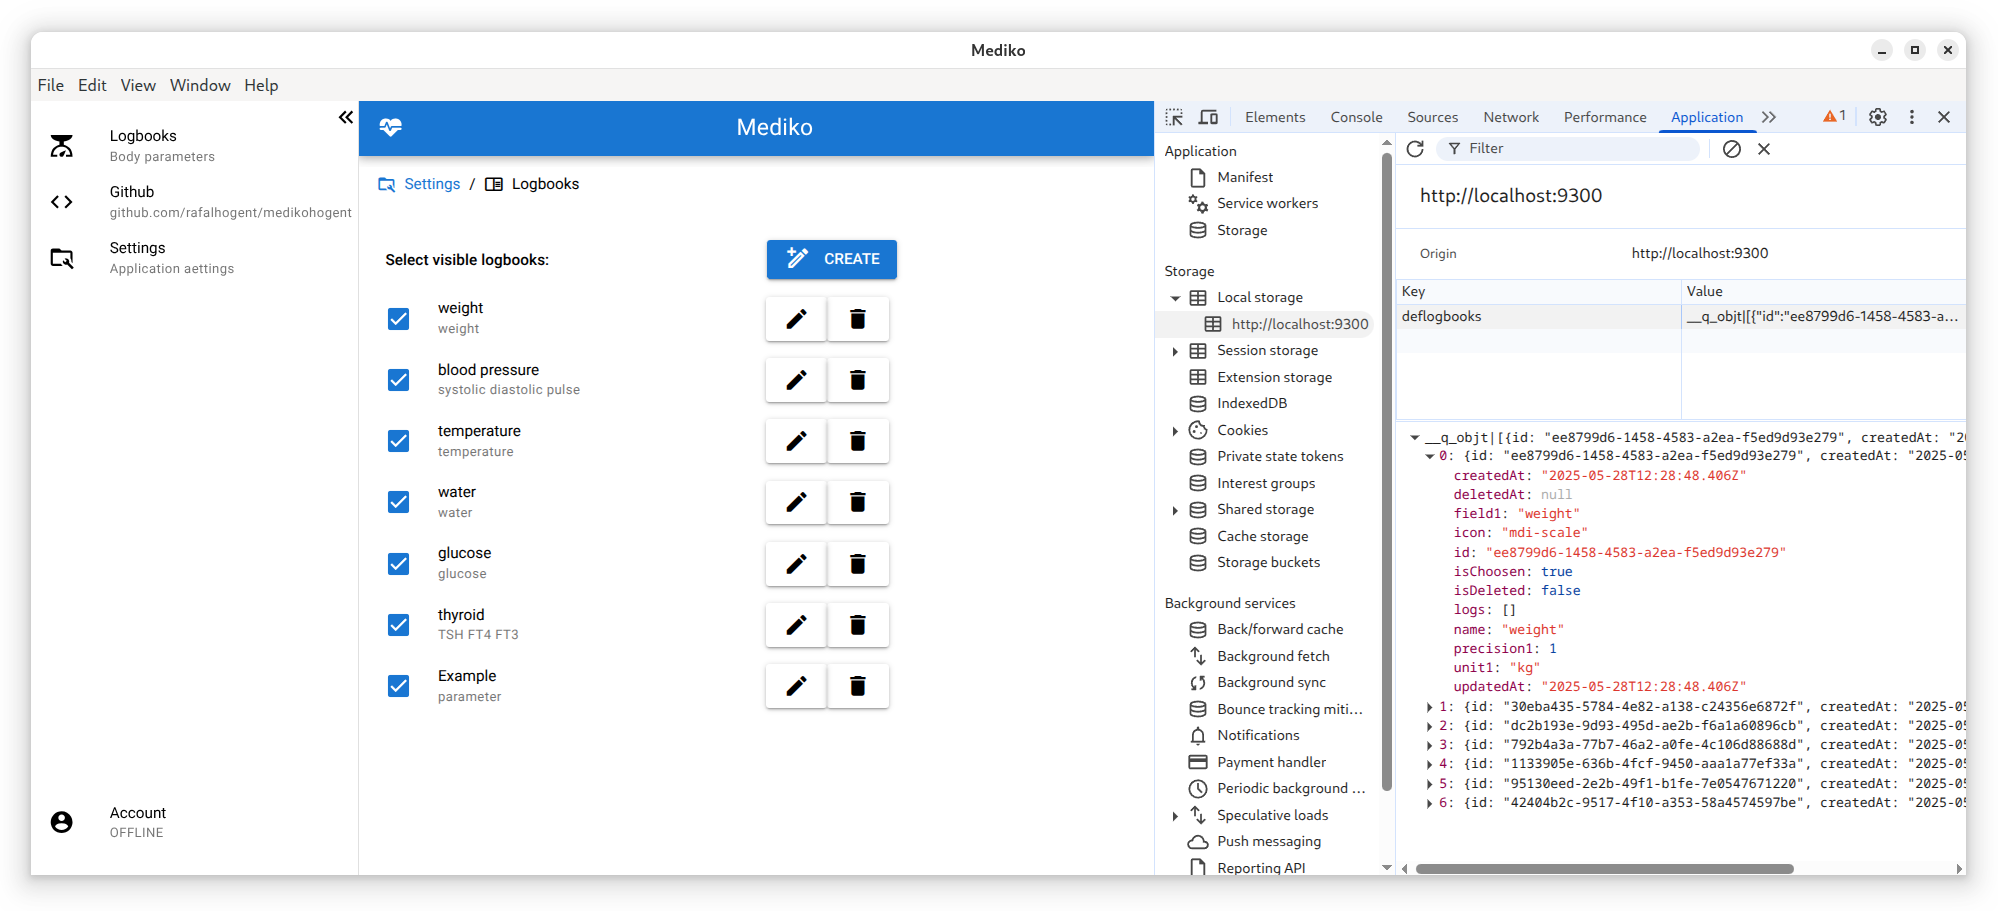
\includegraphics[width=0.8\textwidth]{electron-linux.png}
    \caption[Electron development mode]{\label{fig:electronlinux} Electron Application in development mode running on Wayland session on Fedora Linux x86/x64. Created logbooks are visible in the Local Storage }
\end{figure}



\section{{Building for Windwows}}%
\label{sec:windows}

To build Electron for Microsoft Windows under Linux there was a VirtualBox \autocite{VBox} software used to start virtual machine with some prerequisites like vscode, git, npm already installed. On Windows, developing an Electron App can be started as on Linux with the following command:

\begin{verbatim}
    quasar dev -m electron
\end{verbatim}


\begin{figure}[H]
    \centering
    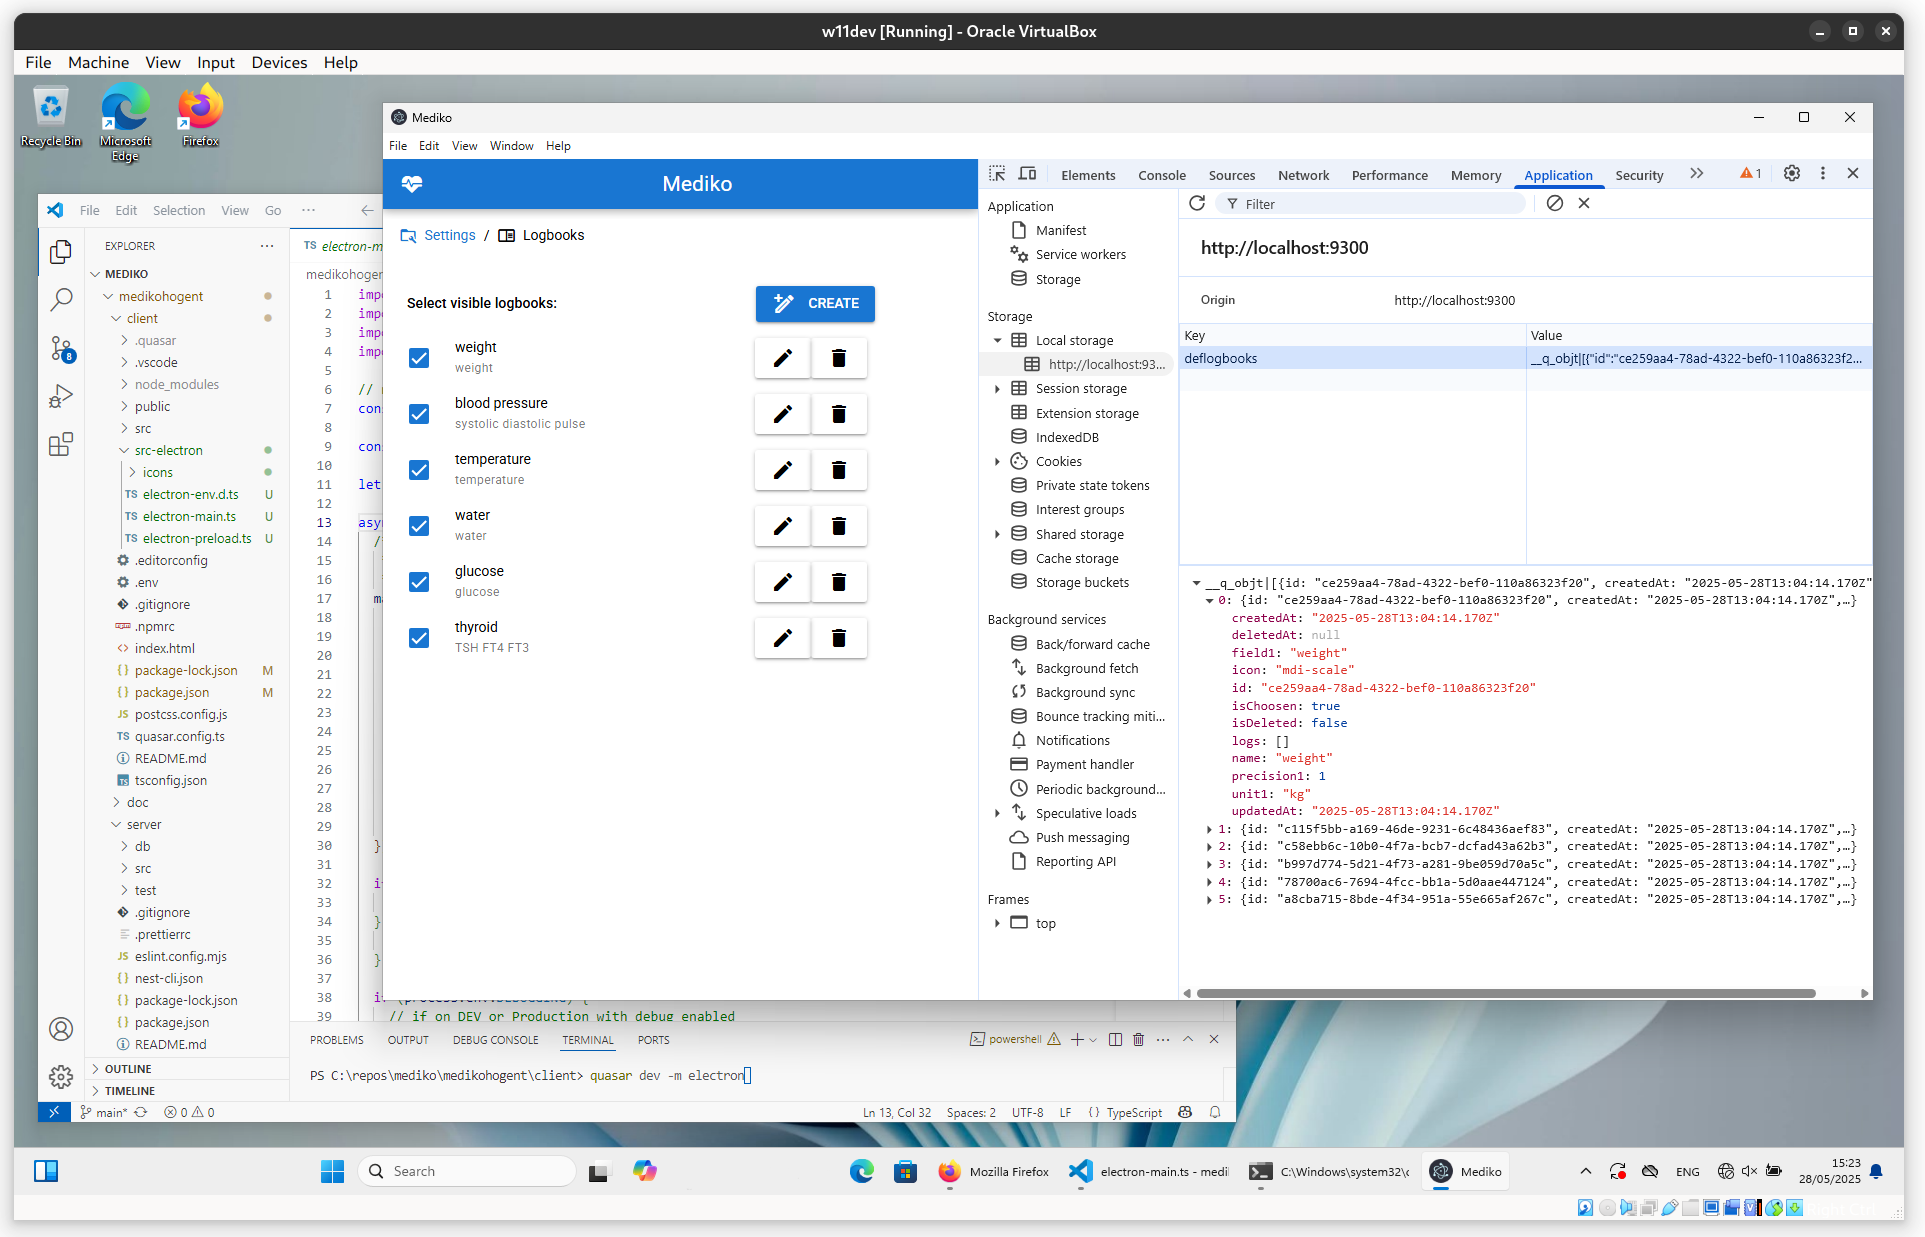
\includegraphics[width=0.8\textwidth]{windows-vm.png}
    \caption[Electron on Windows virtual machine]{\label{fig:windowsvbox} Electron development running on Windwos 11 in Virtualbox }
\end{figure}


\section{{Building Mobile App}}%
\label{sec:mobile}

Making builds fro Android requires some extra preparation work. The first step is to make sure you got the Cordova CLI installed and the necessary SDKs.
\begin{verbatim}
    npm install -g cordova
\end{verbatim}

After this step is done we need to install the Android platform SDK and Android Studio.  

It is also necessary to add environment variables to let the development kit know, where required packages are located.

\begin{listing}[H]
    \begin{minted}{shell}
export ANDROID_HOME="$HOME/Android/Sdk"
export ANDROID_SDK_ROOT="$HOME/Android/Sdk"
export PATH=$PATH:$ANDROID_SDK_ROOT/tools; PATH=$PATH:$ANDROID_SDK_ROOT/platform-tools
    \end{minted}
\caption[Environmental variables for Android SDK on Linux and macOS]{Environmental variables for Android Development on Linux and macOS}
\end{listing}

After installation of Android Studio with correctly configured SDK, an Android virtual machine was created (Medium Phone API 35, Android 15).

In order to develop/build a Mobile app, the Cordova mode has to be added to Quasar project with the following command: 

\begin{verbatim}
    quasar mode add cordova
\end{verbatim}

Development server can be started with the following command, target platforms get installed automatically on demand by Quasar CLI.

\begin{verbatim}
    quasar dev -m cordova -T [android|ios]
\end{verbatim}

\begin{figure}[H]
    \centering
    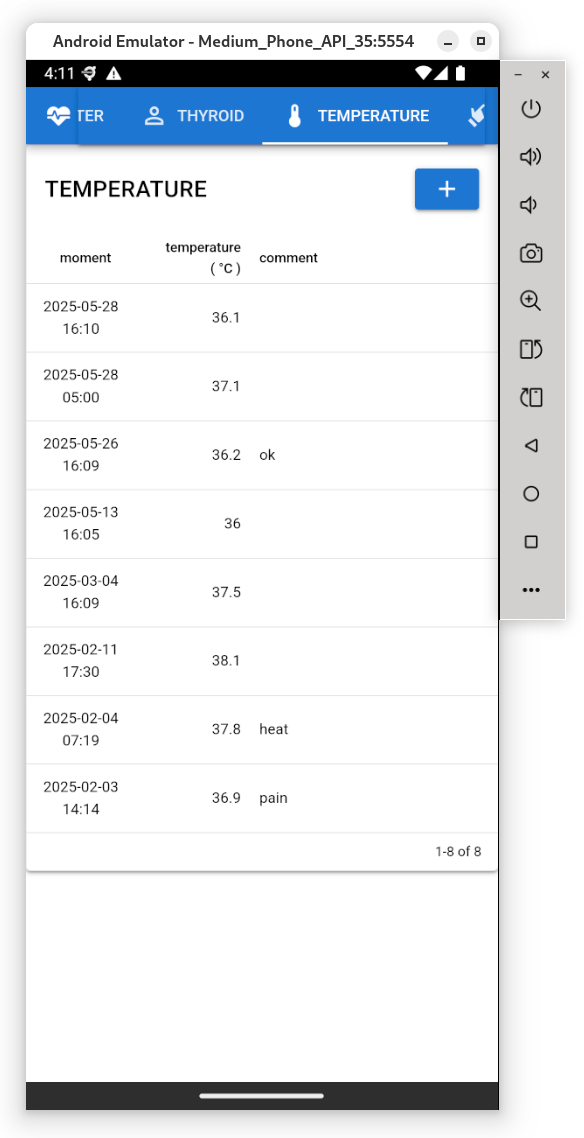
\includegraphics[width=0.3\textwidth]{android.png}
    \caption[Cordova App running on Android Emulator]{\label{fig:android} Cordova App running on Android Emulator }
\end{figure}